\documentclass[12pt, titlepage]{article}
\usepackage[shortlabels]{enumitem}
\usepackage{comment}
\usepackage{booktabs}
\usepackage{tabularx}
\usepackage{hyperref}
\usepackage{float}
\usepackage{soul}
\usepackage{changepage}
\usepackage{graphicx}
\hypersetup{
    colorlinks,
    citecolor=blue,
    filecolor=black,
    linkcolor=red,
    urlcolor=blue
}
\usepackage[round]{natbib}
\usepackage[dvipsnames]{xcolor}

%% Comments

\usepackage{color}

\newif\ifcomments\commentstrue %displays comments
%\newif\ifcomments\commentsfalse %so that comments do not display

\ifcomments
\newcommand{\authornote}[3]{\textcolor{#1}{[#3 ---#2]}}
\newcommand{\todo}[1]{\textcolor{red}{[TODO: #1]}}
\else
\newcommand{\authornote}[3]{}
\newcommand{\todo}[1]{}
\fi

\newcommand{\wss}[1]{\authornote{blue}{SS}{#1}} 
\newcommand{\plt}[1]{\authornote{magenta}{TPLT}{#1}} %For explanation of the template
\newcommand{\an}[1]{\authornote{cyan}{Author}{#1}}

%% Common Parts

\newcommand{\progname}{ProgName} % PUT YOUR PROGRAM NAME HERE
\newcommand{\authname}{Team \#, Team Name
\\ Student 1 name
\\ Student 2 name
\\ Student 3 name
\\ Student 4 name} % AUTHOR NAMES                  

\usepackage{hyperref}
    \hypersetup{colorlinks=true, linkcolor=blue, citecolor=blue, filecolor=blue,
                urlcolor=blue, unicode=false}
    \urlstyle{same}
                                


\begin{document}

\title{System Verification and Validation Plan for \progname{}} 
\author{\authname}
\date{\today}
	
\maketitle

\pagenumbering{roman}

\begin{table}[H]
  \caption{\bf Revision History}
  \begin{tabularx}{\textwidth}{p{2.5cm}p{2.5cm}X}
  \toprule {\bf Date} & {\bf Developer} & {\bf Notes/Changes}\\
  \midrule
  Oct 31, 2022 & Timothy Chen & Added to 5.2, 5.3, 7.2\\
  Oct 31, 2022 & Edwin Do & Added section 4 for V\&V Plan\\
  Nov 1, 2022 & Abdul Nour Seddiki & Added to 5.1, 5.3\\
  Nov 2, 2022 & Joseph Braun & Added Section 3\\
  Nov 2, 2022 & Edwin Do & Added more content to section 4 \\
  \bottomrule
  \end{tabularx}
  \end{table}
  

\newpage

\tableofcontents

\listoftables
\wss{Remove this section if it isn't needed}

\listoffigures
\wss{Remove this section if it isn't needed}

\newpage

\section{Symbols, Abbreviations and Acronyms}

\renewcommand{\arraystretch}{1.2}
\begin{tabular}{l l} 
  \toprule		
  \textbf{symbol} & \textbf{description}\\
  \midrule 
  T & Test\\
  SRS & Software Requirements Specifications \\
  VS & Visual Studio\\
  UWP & Universal Windows Platform\\
  \bottomrule
\end{tabular}\\

\wss{symbols, abbreviations or acronyms -- you can simply reference the SRS
  \citep{SRS} tables, if appropriate}

\newpage

\pagenumbering{arabic}

\section{General Information}

\subsection{Summary}

The purpose of this document is to provide a detailed plan for the testing of our system. This will include:
\begin{itemize}
  \item Verification and Validation Plan
  \item System Test Description
  \item Unit Test Description
\end{itemize}

\subsection{Objectives}

The objectives of testing are to ensure that all functional and non-functional requirements of the system are being met. It is important to include both unit tests as well as system tests, as issues may arise when components are connected together in the system. 

\subsection{Relevant Documentation}

Relevant documentation includes:
\begin{itemize}
  \item SRS
  \item MIS
  \item MG
\end{itemize}

\section{Plan}
% RUBRIC
% 'Team member's roles for testing are clear;  
% This may involve switching roles between verification tasks 
% (say between SRS verification, hardware verification, and code verification).  
% Clear, specific and feasible plan for SRS verification; 
% Clear specific and feasible plan for Design verification; 
% Clear specific and feasible plan for implementation verification.  
% Automated testing and verification tools are specific.  
% Software validation plan is clear, specific and feasible.

% \wss{Introduce this section.   You can provide a roadmap of the sections to
%   come.}

  In this section of planning, it will outline our approaches to cover the requirements 
  outlined in various areas such as the SRS document, Hazard analysis document, our implementation and design. 
  Tools that will be used for automated unit testing and linting will also be introduced.\\

  The following topics will be covered:

  \begin{itemize}
    \item The verification and validation team along with their respective responsibilities
    \item Our approach towards the SRS Verification plan
    \item Our approach towards the Design Verification plan
    \item Implementation verification plan
    \item Any testing and verification tools we plan to use
  \end{itemize}


\subsection{Verification and Validation Team}

% \wss{You, your classmates and the course instructor.  Maybe your supervisor.
%   You shoud do more than list names.  You should say what each person's role is
%   for the project.  A table is a good way to summarize this information.}

  Below is a table outlining the members of the Verification and Validation team along with their respective responsibilities.
  Note that the listed responsibilities are only used as a guideline, responsibilities can shift between team members on a as-per-needed basis.

  \begin{table}[H]
    \centering
    \caption{Team and Responsibilities}
    \label{my-label}
    \begin{tabular}{|c|c|c|}
      \hline
      \textbf{Team Member} & \textbf{Role Name} & \textbf{Responsibilities}   \\ \hline
      Edwin Do & 
      \begin{tabular}{@{}c@{}}Software and SRS Tester\end{tabular} & 
      \begin{tabular}{@{}c@{}}Ensures that all requirements are valid \\ 
        and verified under the scope of software \\
        capabilities in this project and the SRS\end{tabular} \\ \hline
      
      Timothy Chen & 
      \begin{tabular}{@{}c@{}}Software Tester\end{tabular} & 
      \begin{tabular}{@{}c@{}}Ensures that all requirements are met \\ 
        and verified under the scope of software \\
        capabilities in this project\end{tabular} \\ \hline
      
      Tyler Magarelli & 
      \begin{tabular}{@{}c@{}}Software Tester\end{tabular} & 
      \begin{tabular}{@{}c@{}}Ensures that all requirements are met\\ 
        and verified under the scope of software \\
        capabilities in this project\end{tabular} \\ \hline
      
      Joseph Braun & 
      \begin{tabular}{@{}c@{}}Hardware Tester\end{tabular} & 
      \begin{tabular}{@{}c@{}}Ensures that all requirements are met \\ 
        and verified under the scope of hardware \\
        capabilities in this project\end{tabular} \\ \hline
      
      Abdul Nour Seddiki & 
      \begin{tabular}{@{}c@{}}Hardware Tester\end{tabular} & 
      \begin{tabular}{@{}c@{}}Ensures that all requirements are met \\ 
        and verified under the scope of hardware \\
        capabilities in this project\end{tabular} \\ \hline

      Dr. Hatem Zurob & 
      \begin{tabular}{@{}c@{}}Supervisor\end{tabular} & 
      \begin{tabular}{@{}c@{}}Ensures that all requirements are valid \\ 
        and meets the expected result\end{tabular} \\ \hline
    \end{tabular}
  \end{table}

\subsection{SRS Verification Plan}

% \wss{List any approaches you intend to use for SRS verification.  This may just
%   be ad hoc feedback from reviewers, like your classmates, or you may have
%   something more rigorous/systematic in mind..}

% \wss{Remember you have an SRS checklist}

\noindent To verify our SRS, our team intends on revisiting the SRS document on a bi-weekly basis to verify that 
the requirements are up to date and in sync with the project goal. This will also allow us to cover any
newly discover risks or hazards which will also be reflected in the Hazard Analysis document. Any new changes
within the two week window will be noted and discussed at the end to see if additional changes to the SRS document 
would be necessary. At each bi-weekly review, the team also plans on using the SRS checklist as a guideline throughout
the meeting.\\

\noindent  In addition, the team will use ad hoc feedback from reviewers such as classmates from our 4GA6 Capstone class as well
as instructor, supervisor and teaching assistants. This will act as a supplementary addition if any element of the SRS 
is out of date or missing.

\subsection{Design Verification Plan}

Our plans to verify our design document includes using the MIS checklist and reviews from our classmates. 
The MIS checklist will help our team ensure that the design logic helps us meet the requirements specified in 
the SRS document and cover any hazards or risks outlined in the Hazard analysis. The team will conduct an internal 
design review, by going over all the outlined requirements, risks and hazards and verifiying that the design does not
contain any logical flaws to the best of our abilities. \\

\noindent  In addition, the team will use the feedback from reviewers such as classmates from our 4G06 Capstone class as well
as instructor, supervisor and teaching assistants. This will help further assist our team to ensure that the design is free from 
any logical flaws and is able to help meet the outlined requirements. 

% \wss{Plans for design verification}

% \wss{The review will include reviews by your classmates}

% \wss{Remember you have MG and MIS checklists}

\subsection{Implementation Verification Plan}

% [Point to other tests and unit testing plan]

Throughout the development phase of this project, the team will use GitHub Issues and pull requests to implement
various features. Each pull request will require at least two other team members to inspect and review the code 
ensuring that it meets the requirement and design discussed. A pipeline can also be implemented in GitHub to ensure that
the build in the main branch is always stable. Unit tests will also be used to ensure that the implementation of the product
is verified. 

% \wss{You should at least point to the tests listed in this document and the unit
%   testing plan.}

% \wss{In this section you would also give any details of any plans for static verification of
%   the implementation.  Potential techniques include code walkthroughs, code
%   inspection, static analyzers, etc.}

\subsection{Automated Testing and Verification Tools}

The final product will be an Universal Windows Platform (UWP) application built using Microsoft Visual Studio (VS) in C\# and XAML. \\

\noindent Majority of the project's testing will be conducted within VS. 
For unit testing, the team will use the built-in features of Unit Test Applications in VS to create unit tests projects and units tests.\\

\noindent Code coverage tests is also covered within the suite of tools available within VS. The team will be able to create testing suites and 
unit tests for the VS project. The team also plans on using the results of the code coverage
tests to identify which portion of the project's code not covered by our tests. Uncovered blocks of code can be colour-coded to signify to 
the developer that no current test covers that block of code. Other metrics such as number of lines covered, \% of a block covered will be 
summarized per code coverage project to help indicate where more testing efforts are needed. \\

\noindent Using Visual Studio's IDE extensions, the team plans on using SonarLint and CSharpier as its linter and formatting tool for C\# respectively. 

% \wss{What tools are you using for automated testing.  Likely a unit testing
%   framework and maybe a profiling tool, like ValGrind.  Other possible tools
%   include a static analyzer, make, continuous integration tools, test coverage
%   tools, etc.  Explain your plans for summarizing code coverage metrics.
%   Linters are another important class of tools.  For the programming language
%   you select, you should look at the available linters.  There may also be tools
%   that verify that coding standards have been respected, like flake9 for
%   Python.}

% \wss{The details of this section will likely evolve as you get closer to the
%   implementation.}

\subsection{Software Validation Plan}

To verify that the software will work as intended and designed, the team will use the sample 
data provided by Dr. Zurob and see if the results are within a reasonable margin of error. This
sample data is obtained from a collection of existing materials with known results. If the actual 
results are outside a reasonable range, then the team shall conclude that the results are not valid. 


% Use sample data provided by Dr.Zurob to ensure accuracy of data 

% \wss{If there is any external data that can be used for validation, you should
%   point to it here.  If there are no plans for validation, you should state that
%   here.}

\section{System Test Description}
	
\subsection{Tests for Functional Requirements}

\begin{enumerate}[{FR-T}1.]
    \item Control: Dynamic \& Manual \\
    Initial State: Entire system is set up and the application is running.\\
    Input: Developers will set up a sample and demonstrate the main function of the application.\\
    Output: The application shall display the voltage, the current, the temperature and measure the conductivity of sample materials in real-time. Updates to values on the measurement tools should match with updates on the application and changes to the value of conductivity. \\
    Test Case Derivation: Since the measurement tools are using a unified communication bus with the control computer, measurements are expected to be synchronised and displayed in real-time.\\
    How test will be performed: Test will be performed by developers. Simultaneously monitoring both the values displayed on the external measurement tools and the values in the application and observing for latency in the display and calculation.
    
    \item Control: Dynamic \& Manual\\
    Initial State: Entire system is set up and the application is running.\\
    Input: Developers will set up a sample and perform thermal treatment on it.\\
    Output: The application shall make note of critical changes in conductivity.\\
    Test Case Derivation: While the application is constantly monitoring the state of conductivity of samples in real-time, any major change in the conductivity indicates a transition in the phase of the material.\\
    How test will be performed: Test will be performed by developers. Performing thermal treatment and observing changes in conductivity as calculated by the application.
    
    \item Control: Dynamic \& Manual\\
    Initial State: Entire system is set up and the application is running.\\
    Input: Developers will modify the setting that controls the data sampling rate in the application.\\
    Output: The sampling rate of inputs is modified. Therefore, the display rate of inputs and outputs is going to change.\\
    Test Case Derivation: The application is expected to be able to sample the data at variable rates, either by changing the actual rate of data acquisition or by changing the interval at which the data is displayed and analysed.\\
    How test will be performed: Test will be performed by developers, manually testing this function of the system. 
    
    \item Control: Dynamic \& Manual\\
    Initial State: Entire system is set up and the application is running.\\
    Input: Developers will set up a sample and perform thermal treatment on it.\\
    Output: The application shall automatically calculate the slopes of resistivity-temperature in the phase change diagram, identify changes in these slopes and attributing slope changes to phase transitions. This information is highlighted with appropriate phase transition labels.\\
    Test Case Derivation: While the application is constantly monitoring the resistivity of samples in real-time, major changes in the resistivity to temperature ratios correlate to phase changes of the material.\\
    How test will be performed: Test will be performed by developers. Performing thermal treatment and observing notifications and labels on graphs or logs made by the application.
    
    \item Control: Dynamic \& Manual\\
    Initial State: Entire system is set up and the application is running.\\
    Input: Developers will prompt a wireless connection to control computer and navigate the application.\\
    Output: The application is able to be controlled using a proxy/web application.\\
    Test Case Derivation: The control computer is expected to be connected to the network so that when the system is set up the application is operable remotely.\\
    How test will be performed: Test will be performed by developers communicating remotely with the control computer.  
\end{enumerate}

\subsection{Tests for Nonfunctional Requirements}

\subsubsection{Appearance Test}

\begin{adjustwidth}{2.2em}{0pt}
\begin{enumerate}[{NF-AT}1.]
    \item Type: Static \& Manual \\
    Initial State: Application home screen will be open.\\
    Input/Condition: Users will explore the application then take a survey.\\
    Output/Result: Survey result will indicate 90 percent of users feel application is uncomplicated. \\
    How test will be performed: Test will be performed by the user. They will receive a survey with a question. If 90 percent of users inidicate a 1 out of 5, it will be considered successful. (Appendix)
    
    \item Type: Static \& Manual\\
    Initial State: Application home screen will be open.\\
    Input/Condition: Developers will navigate the application and explore all sections.\\
    Output/Result: Developers will ensure all section of the application is in English.\\
    How test will be performed: Test will be performed by developers. 
  \end{enumerate}
\end{adjustwidth}

\subsubsection{Usability Test}

\begin{adjustwidth}{2.2em}{0pt}
\begin{enumerate}[{NF-UT}1.]

How test will be performed: 

    \item Type: Dynamic \& Automated\\
    Initial State: Application home screen will be open.\\
    Input/Condition: Invalid and edge case parameters will be enter into the application.\\
    Output/Result: Application will flag the parameters that are not accepted and prevent the program from running.\\
    How test will be performed: Test will be performed by a script which will enter and check for the flag messages after parameters have been given.

    \item Type: Dynamic \& Manual\\
    Initial State: Application will be closed.\\
    Input/Condition: Users will be ask to open the application and perform a task. User then will be asked to return the next day to perform the same task.\\
    Output/Result: Time from the users opening the application to interacting with it should be within 5 seconds.\\
    How test will be performed: Test will be performed by the users. The test will pass only if the time is within 5 seconds and the task the user is asked to complete is completed without any mistakes the second time.

    \item Type: Static \& Manual\\
    Initial State: Application will be open.\\
    Input/Condition: Developers will navigate and explore the application.\\
    Output/Result: No calculations will be found when exploring the application. \\
    How test will be performed: Test will be performed by the developers.

    \item Type: Static \& Manual\\
    Initial State: Research device will not have the application on it.\\
    Input/Condition: Users will install the application on the device.\\
    Output/Result: Application capacity on the device will be less than 8 GB.\\
    How test will be performed: Test will be performed by the users.

    \item Type: Staic \& Manual\\
    Initial State: Application will be installed on the device.\\
    Input/Condition: Users will set up the application with the measurement equipments according to instructions provided.\\
    Output/Result: Application will not indicate further set up required after the initial set up of the measurement devices on the first uses.\\
    How test will be performed: Test will be performed by users. User will be ask to set up the measurement equipment. The next time the user uses the appliaction, there will be no inidication that there will be a need to perform further set up. 
\end{enumerate}
\end{adjustwidth}

\subsubsection{Performance Test}

\begin{adjustwidth}{2.2em}{0pt}
\begin{enumerate}[{NF-PT}1.]
    \item Type: Dynamic \& Automated\\
    Initial State: Measurement devices will be connected to sample and to device with application open.\\
    Input/Condition: Start thermal treatment of sample.\\
    Output/Result: Should return 100 readings a second for 95 precent of the time with the lowest reading being 98 per second.\\
    How test will be performed: Test will be performed by a script to start the treatment while measuring the readings per second. 
    
    \item Type: Dynamic \& Automated\\
    Initial State: Application will have defualt parameters.\\
    Input/Condition: Parameters will be changed\\
    Output/Result: Application will relfect changes by within 1 second for 95 percent of the time with the longest time being 2 seconds.\\
    How test will be performed: Test will be performed by a script where parameters will be changed and the change will be timed and verified.

    \item Type: Dynamic \& Automated\\
    Initial State: Measurement devies will be connected to device.\\
    Input/Condition: Thermal treatment sample data will be read into the device.\\
    Output/Result: The sample reading from the thermal treatment will be accurate to 3 decminal places 99.99 percent of the time.\\
    How test will be performed: Test will be performed by a script where the data being read in will be compared to an exising data set of the same sample with the same parameters. The data will be identical for 99.99 percent of the readings.

    \item Type: Dynamic \& Automated\\
    Initial State: Application will be open with measuremnt devices connceted.\\
    Input/Condition: Readings for thermal treatment sample.\\
    Output/Result: The calculations displayed on the application will be accurate to 3 decimal places for 99.99 percent of the time.\\
    How test will be performed: Test will be performed by a sscript performing the caluations and comparing the result to the result on the application.

    \item Type: Dynamic \& Automated\\
    Initial State: Application will be closed.\\
    Input/Condition: Application will be opened and have modification applied to the it.\\
    Output/Result: The application will be up and running 99 percent of the time.\\
    How test will be performed: Test will be performed by a script making modifications on the application throughout 12 hours and seeing if the application gives a healthly response for 99 percent of the time.
\end{enumerate}
\end{adjustwidth}

\subsubsection{Operational Test}

\begin{adjustwidth}{2.2em}{0pt}
\begin{enumerate}[{NF-OT}1.]
    \item Type: Static \& Manual\\
    Initial State: Application will be open with keyboard and mouse connected to the device.\\
    Input/Condition: User will interact with the application with mouse and keyboard.\\
    Output/Result: Application will reflect inputs provided by mouse and keyboard.\\
    How test will be performed: Test will be performed by the users.
    
    \item Type: Static \& Manual\\
    Initial State: Application will be uninstalled from the device.\\
    Input/Condition: Users will be asked to installed the application.\\
    Output/Result: Feedback surveys from the installtion should indicate the installation was simple for 90 percent of of the users.\\
    How test will be performed: Test will be performed by the user. User will be given a survey a question where 1 being simple and 5 being difficult. If 90 percent of users answer 1, it will be considered a success.
\end{enumerate}
\end{adjustwidth}

\subsubsection{Maintainability/Support Test}

\begin{adjustwidth}{2.2em}{0pt}
\begin{enumerate}[{NF-MT}1.]
    \item Type: Static \& Manual\\
    Initial State: Application will be uninstalled for device.\\
    Input/Condition: Application will be installed on the device and connected to measurement devices.\\
    Output/Result: The applications functions will be verified and ensure it is performing smoothly on the device.\\
    How test will be performed: Test will be performed by the developer installing the application onto the  lab computer running window 7.
\end{enumerate}
\end{adjustwidth}

\subsubsection{Security Test}

\begin{adjustwidth}{2.2em}{0pt}
\begin{enumerate}[{NF-ST}1.]
    \item Type: Static \& Manual\\
    Initial State: Application will be open on device.\\
    Input/Condition: User will attempt to inject data or modify parameters they do not have permission for.\\
    Output/Result: Application will have a indicator inform user does not have permission.\\
    How test will be performed: Test will be performed by users who do not have certain permissions.
    
    \item Type: Static \& Manual\\
    Initial State: Application will be open on device.\\
    Input/Condition: User will be asked to change hidden settings and calculations.\\
    Output/Result: Changes should be accepted and saved by the application. Will be reflected on the application interface.\\
    How test will be performed: Test will be performed by users who have permission to access these settings/parameters.
\end{enumerate}
\end{adjustwidth}

\subsubsection{Cultural Test}

\begin{adjustwidth}{2.2em}{0pt}
\begin{enumerate}[{NF-CT}1.]
    \item Type: Static \& Manual\\
    Initial State: Application will be open on device.\\
    Input/Condition: Users will explore the appliaction then take a survey \\
    Output/Result: Result from survey will return a score of 8.\\
    How test will be performed: Test will be performed by users which will take a survey after interacting with the application, 1 being inappropriate and 10 being appropriate. 
\end{enumerate}
\end{adjustwidth}

\subsubsection{Health and Safety Test}

\begin{adjustwidth}{2.2em}{0pt}
\begin{enumerate}[{NF-HT}1.]
    \item Type: Static \& Manual\\
    Initial State: Application will be open on device.\\
    Input/Condition: Users will explore the appliaction then take a survey \\
    Output/Result: Result from survey will indicate application interface does not pose any health concerns.\\
    How test will be performed: Test will be performed by the user which will take a survey regarding the interface's colour and design.  
\end{enumerate}
\end{adjustwidth}

\subsection{Traceability Between Test Cases and Requirements}

\begin{table}[H]
	\centering
	\caption{Requirements Traceability}
	\label{my-label}
	\begin{tabular}{|c|c|}
		\hline
		\textbf{Requirements} & \textbf{Tests} \\ \hline
		FR1 & FR-T1 \\ \hline
		FR2 & FR-T2 \\ \hline
		FR3 & FR-T3 \\ \hline
		FR4 & FR-T4 \\ \hline
		FR5 & FR-T5 \\ \hline
		NFR-L1 & NF-AT1 \\ \hline
    NFR-L2 & NF-AT2 \\ \hline
    NFR-U1 & NF-UT1 \\ \hline
    NFR-U2 & NF-UT2 \\ \hline
    NFR-U3 & NF-UT3 \\ \hline
    NFR-U4 & NF-UT4 \\ \hline
    NFR-U5 & NF-UT5\\ \hline
    NFR-U6 & NF-UT6 \\ \hline
    NFR-U7 & NF-UT7 \\ \hline
    NFR-P1 & NF-PT1 \\ \hline
    NFR-P2 & NF-PT2 \\ \hline
    NFR-P3 & NF-PT3 \\ \hline
    NFR-P4 & NF-PT4 \\ \hline
    NFR-P5 & NF-PT5 \\ \hline
    NFR-O1 & NF-OT1 \\ \hline
    NFR-O2 & NF-OT2 \\ \hline
    NFR-O3 & N/A \\ \hline
    NFR-M1 & N/A \\ \hline
    NFR-M2 & NF-MT1 \\ \hline
    NFR-M3 & NF-MT1 \\ \hline
    NFR-S1 & NF-ST1 \\ \hline
    NFR-S2 & NF-ST2 \\ \hline
    NFR-C1 & NF-CT1 \\ \hline
    NFR-H1 & NF-HT1 \\ \hline
    NFR-H2 & NF-HT1 \\ \hline
    NFR-I1 & NF-MT1 \\ \hline
	\end{tabular}
\end{table}


\section{Unit Test Description}

\wss{Reference your MIS and explain your overall philosophy for test case
  selection.}  
\wss{This section should not be filled in until after the MIS has
  been completed.}

\subsection{Unit Testing Scope}

\wss{What modules are outside of the scope.  If there are modules that are
  developed by someone else, then you would say here if you aren't planning on
  verifying them.  There may also be modules that are part of your software, but
  have a lower priority for verification than others.  If this is the case,
  explain your rationale for the ranking of module importance.}

\subsection{Tests for Functional Requirements}

\wss{Most of the verification will be through automated unit testing.  If
  appropriate specific modules can be verified by a non-testing based
  technique.  That can also be documented in this section.}

\subsubsection{Module 1}

\wss{Include a blurb here to explain why the subsections below cover the module.
  References to the MIS would be good.  You will want tests from a black box
  perspective and from a white box perspective.  Explain to the reader how the
  tests were selected.}

\begin{enumerate}

\item{test-id1\\}

Type: \wss{Functional, Dynamic, Manual, Automatic, Static etc. Most will
  be automatic}
					
Initial State: 
					
Input: 
					
Output: \wss{The expected result for the given inputs}

Test Case Derivation: \wss{Justify the expected value given in the Output field}

How test will be performed: 
					
\item{test-id2\\}

Type: \wss{Functional, Dynamic, Manual, Automatic, Static etc. Most will
  be automatic}
					
Initial State: 
					
Input: 
					
Output: \wss{The expected result for the given inputs}

Test Case Derivation: \wss{Justify the expected value given in the Output field}

How test will be performed: 

\item{...\\}
    
\end{enumerate}

\subsubsection{Module 2}

...

\subsection{Tests for Nonfunctional Requirements}

\wss{If there is a module that needs to be independently assessed for
  performance, those test cases can go here.  In some projects, planning for
  nonfunctional tests of units will not be that relevant.}

\wss{These tests may involve collecting performance data from previously
  mentioned functional tests.}

\subsubsection{Module ?}
		
\begin{enumerate}

\item{test-id1\\}

Type: \wss{Functional, Dynamic, Manual, Automatic, Static etc. Most will
  be automatic}
					
Initial State: 
					
Input/Condition: 
					
Output/Result: 
					
How test will be performed: 
					
\item{test-id2\\}

Type: Functional, Dynamic, Manual, Static etc.
					
Initial State: 
					
Input: 
					
Output: 
					
How test will be performed: 

\end{enumerate}

\subsubsection{Module ?}

...

\subsection{Traceability Between Test Cases and Modules}

\wss{Provide evidence that all of the modules have been considered.}
				
\bibliographystyle{plainnat}

\bibliography{../../refs/References}

\newpage

\section{Appendix}

This is where you can place additional information.

\subsection{Symbolic Parameters}

The definition of the test cases will call for SYMBOLIC\_CONSTANTS.
Their values are defined in this section for easy maintenance.


\begin{figure}
  \subsection{Survey Questions}
  \centering
  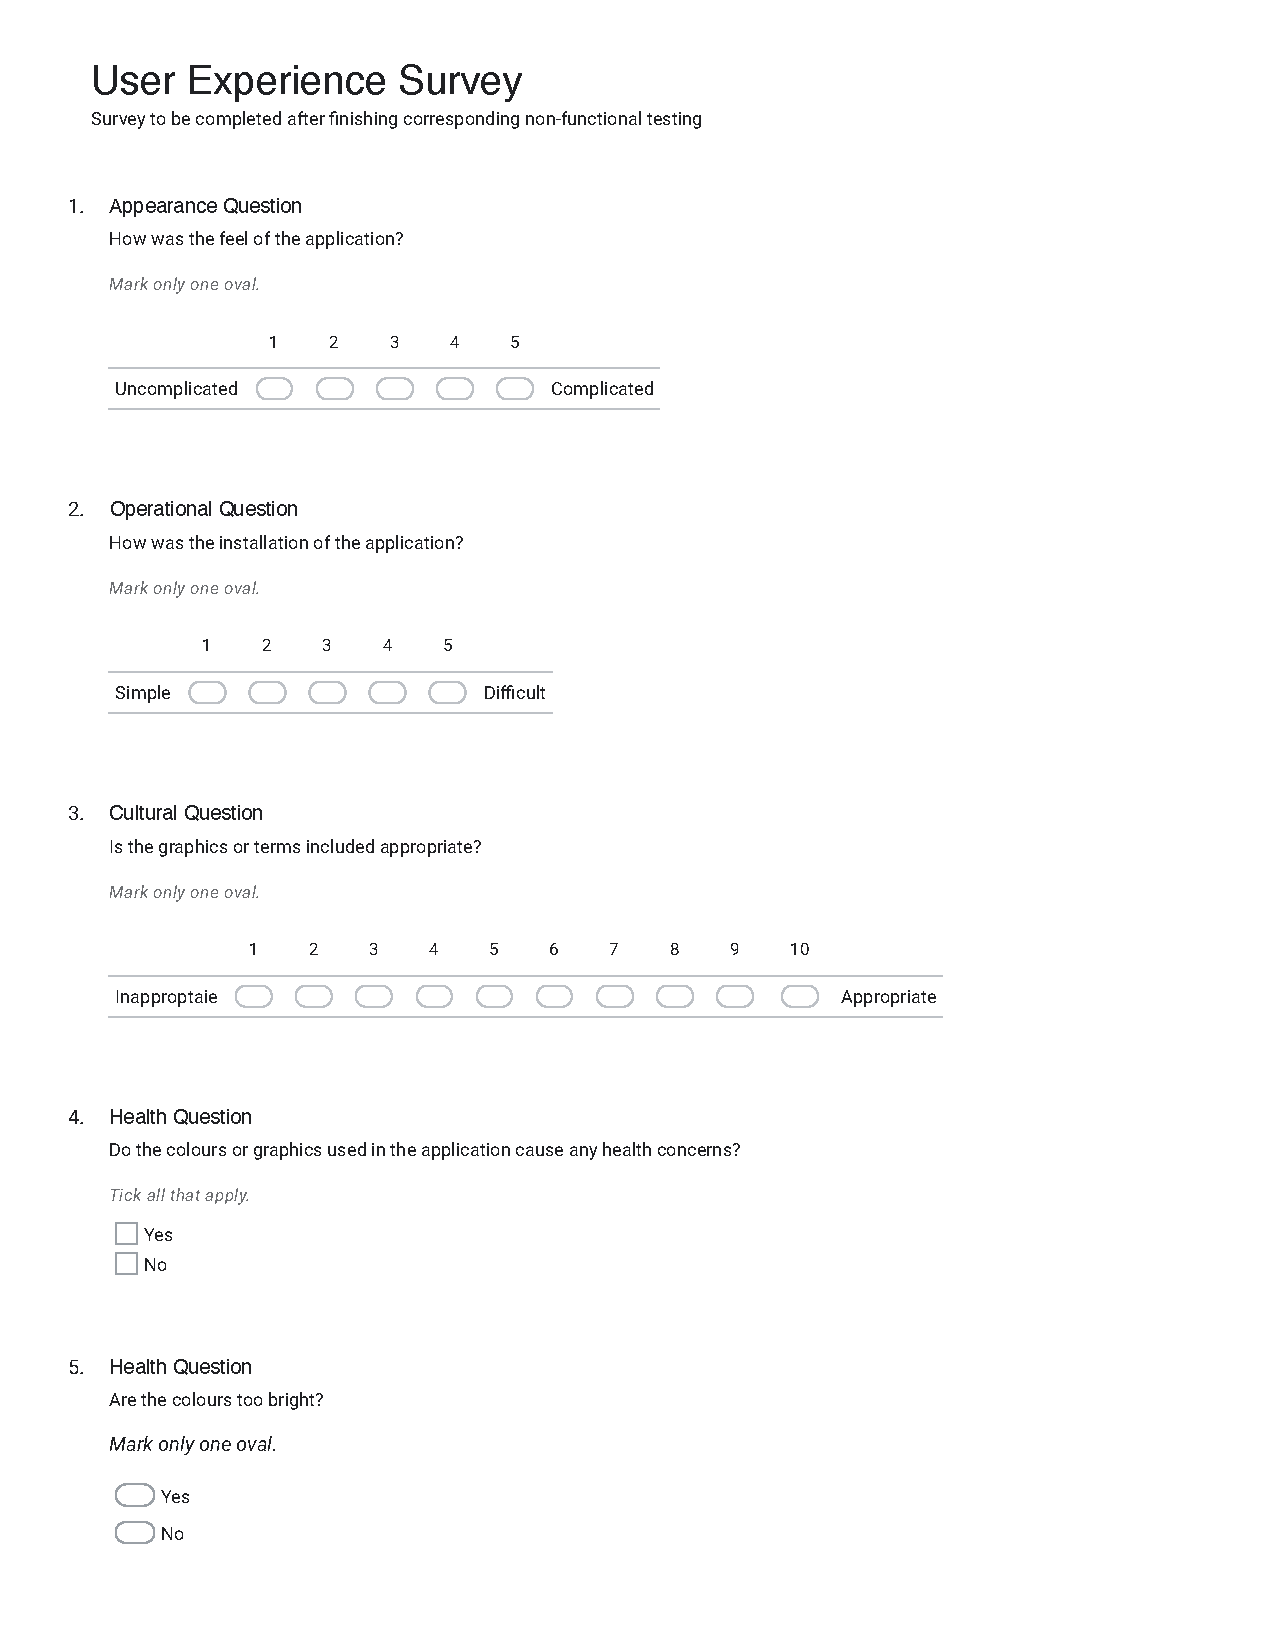
\includegraphics[width=1\textwidth]{User Experience Survey.pdf}
\end{figure}


\newpage{}
\section*{Appendix --- Reflection}

The information in this section will be used to evaluate the team members on the
graduate attribute of Lifelong Learning.  Please answer the following questions:

\begin{enumerate}
  \item 
  \item 
\end{enumerate}

\end{document}